


\chapter{Multirate Signal Processing}

\section{Reference Used}

Chapter 12 from \cite{book_Li_Tan_dsp_fundamentals_and_app}, and chap from \cite{DSP_DimitrisManolakis}.


\section{Downsampling}

We will see now what happen when we do sampling at $T_s$ then do downsampling at a rate of $M \, T_s$ (downsample)


\begin{figure}[h]
\centering
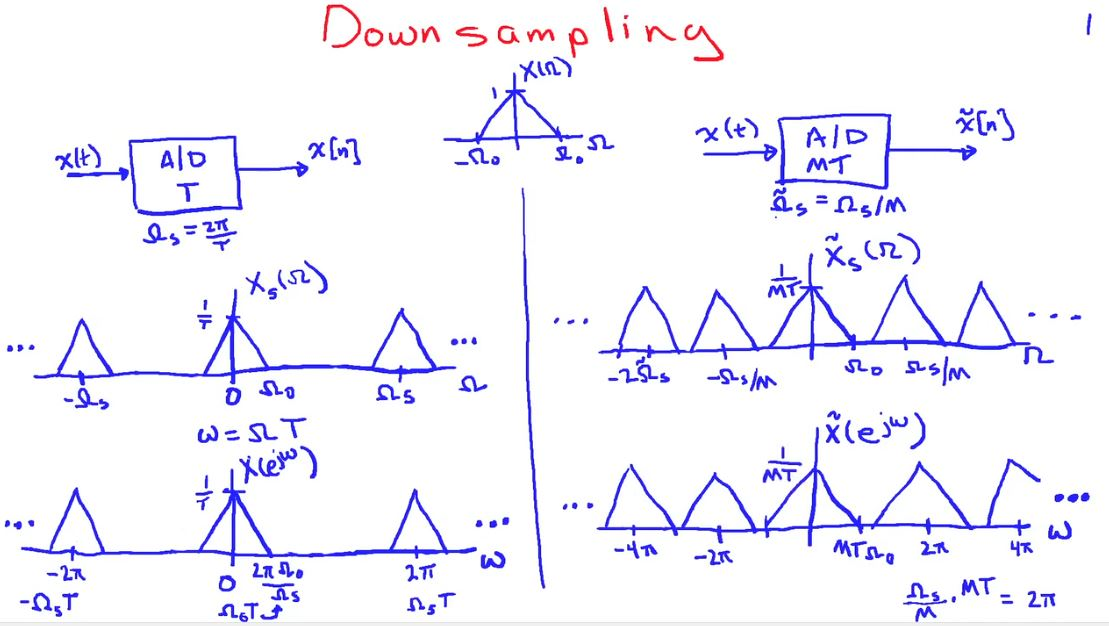
\includegraphics[width = 0.7\textwidth, frame]{Figures/Multirate/downsampling}
\caption{Downsampling effect in the frequency domain}
\label{fig:Multirate:downsampling}
\end{figure} 

\begin{itemize}

\item At a rate of $T_s$, the spectrum get replicated at a multiple of $\omega_s$.

	\begin{itemize}
	\item When we do the frequency mapping $\omega_d \, = \, \omega_c \, \times \, T_s$, the spectrum get replicated at a multiple of 2 $\pi$
	
	
	
	\end{itemize}

\item When doing downsampling:

	\begin{itemize}
	\item $T_{\text{downsample}} \, = \, M \, \times \, T_s$ where $M \, > \, 1 \in \, \mathbb{N}$ and $\omega_{\text{downsample}} \,= \, \displaystyle\frac{\omega_s}{M}$
	
	
	\item The mapping now in frequency is $\omega_d \, = \, \omega_c \, \times \, T_{\text{downsample}}$
	
	
	\item The frequency spectrum in $\omega_c$ now is getting shifted at a multiple of $\displaystyle\frac{\omega_s}{M} $
	
	
	\item In the discrete domain of $-  \pi \, \leq\omega_d \, \leq \,  \pi$, the amplitude is scaled down by $\displaystyle\frac{1}{M \, T_s}$ and the bandwidth is expanded by a factor of $M \, T_s$
	\end{itemize}


\item Aliasing:

If the signal to be downsampled (that is the original signal) has frequency components larger than the new folding frequency $ \leftrightarrow \, f \, > \, \displaystyle\frac{f_s}{2 D}$
aliasing noise will be introduced into the downsampled data.


    \begin{itemize}
        \item To avoid aliasing, the anti-aliaising filter should have a stop frequency edge at $\displaystyle\frac{f_s}{2 \, D}$ (or $\displaystyle\frac{\pi}{D}$ radian in discrete frequency)
    \end{itemize}





\end{itemize}




\subsection{Implementing Downsampling}


\begin{figure}[h]
\centering
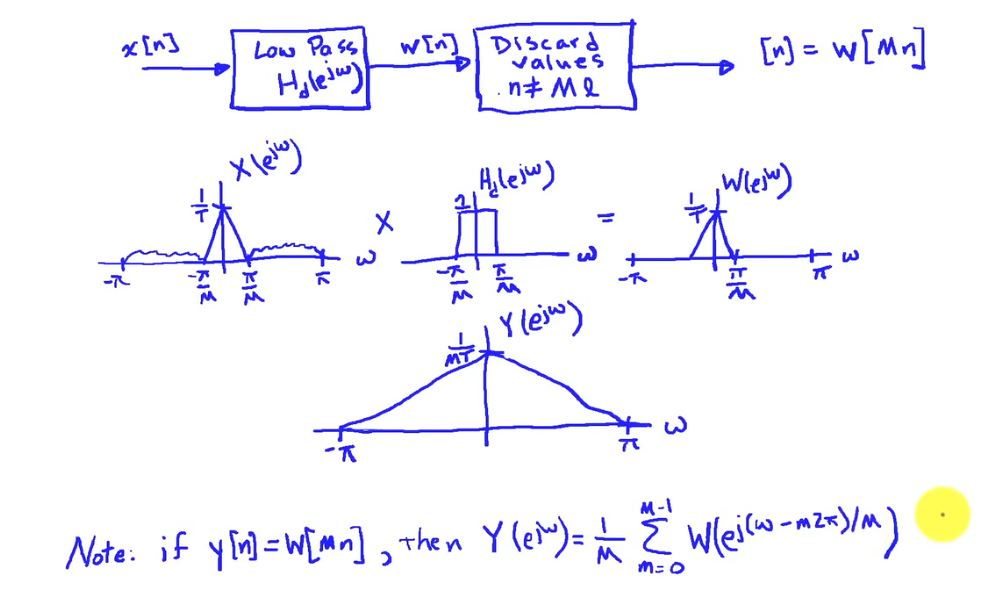
\includegraphics[width = 0.7\textwidth, frame]{Figures/Multirate/implementing_downsampling}
\caption{Implementation of downsampling}
\label{fig:Multirate:implementing_downsampling}
\end{figure} 


\begin{enumerate}

\item Input the discrete signal $x[k]$ in a low pass filter to prevent aliasing 


\item Then we throw the values that are not multiple of $M$

	\begin{itemize}
	\item $y[k] \, = \, w \left[M \, k \right]$: scaling the discrete time axis by a factor of $M$
	
	
	\item We compress the signal in time which means we stretch it in frequency domain: the amplitude spectrum of the signal has stretch out from $\displaystyle\frac{\pi}{M} \, \rightarrow \, \pi$
	
	\item DTFT property for scaling:
	
	
	if $y[k] \, = \, w \left[M \, k \right] \, \rightarrow \, Y(\omega_d) \, = \, \displaystyle\frac{1}{M} \, \displaystyle\sum\limits_{m  \, = \, 0}^{M \, - \, 1} W \left[\, \text{exp}\, \left(\, \displaystyle\frac{j \left(\, \omega_d \, - \, m \, 2 \, \pi \,\right)}{M} \, \right)  \,\right]$
	\end{itemize}


\end{enumerate}

\newpage
\section{Upsampling}

Upsampling is also know as discrete time interpolation.

Effect on spectrum both in continuous time frequency and discrete time frequency is shown in \autoref{fig:Multirate:upsampling}.

\begin{figure}[h]
\centering
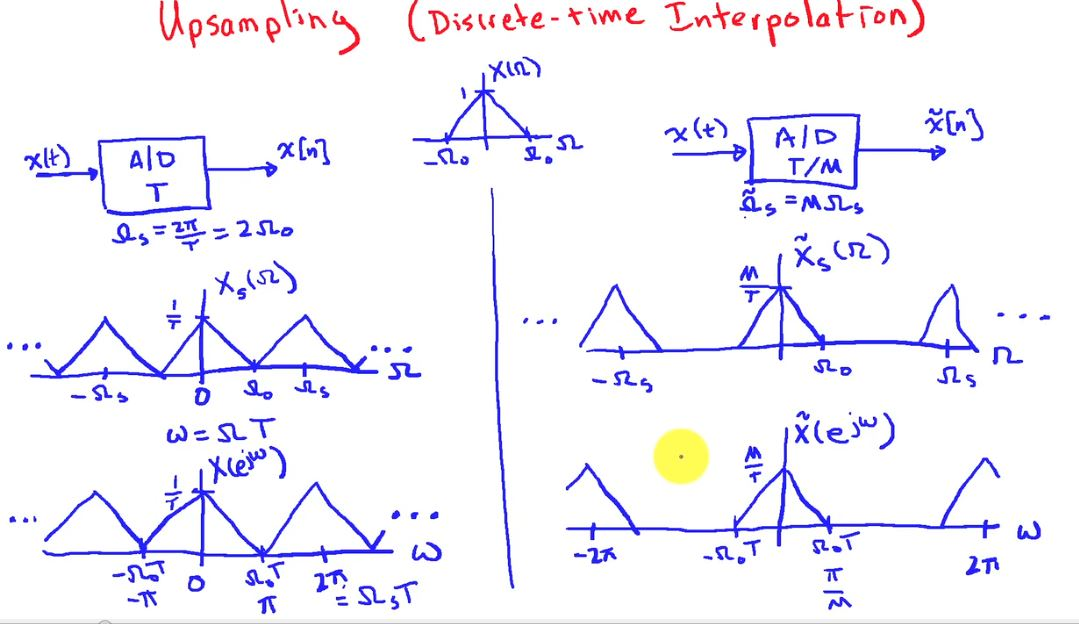
\includegraphics[width = 0.7\textwidth, frame]{Figures/Multirate/upsampling}
\caption{Upsampling effect in the frequency domain}
\label{fig:Multirate:upsampling}
\end{figure} 

\begin{itemize}

\item Opposite to downsampling operation, upsampling compress the spectrum 

\end{itemize}

Example of upsampling in discrete time domain is shown in \autoref{fig:Multirate:upsampling_example}.

\begin{figure}[h]
\centering
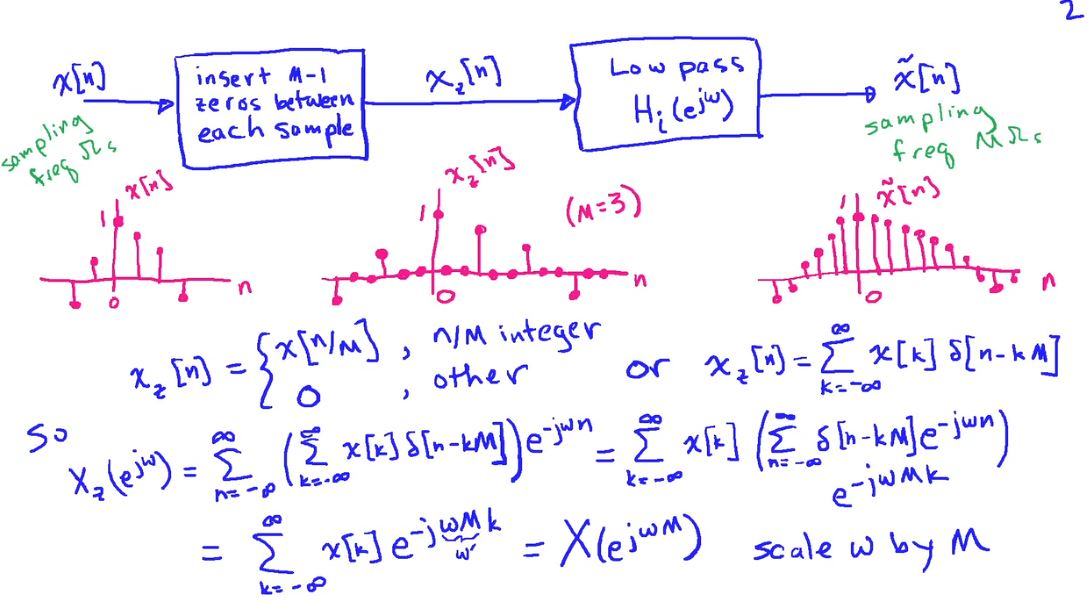
\includegraphics[width = 0.7\textwidth, frame]{Figures/Multirate/upsampling_example}
\caption{Upsampling Example}
\label{fig:Multirate:upsampling_example}
\end{figure} 

\begin{itemize}

\item We add 0 between each sample of the original discrete time $x(k)$ signal such that $\displaystyle\frac{n}{M} \in \mathbb{N}$

\item Then we filter the signal by a low pass filter

\end{itemize}


\newpage
Example of the process in the DTFT spectrum is shown in \autoref{fig:Multirate:upsampling_example_spectrum}.

\begin{figure}[h]
\centering
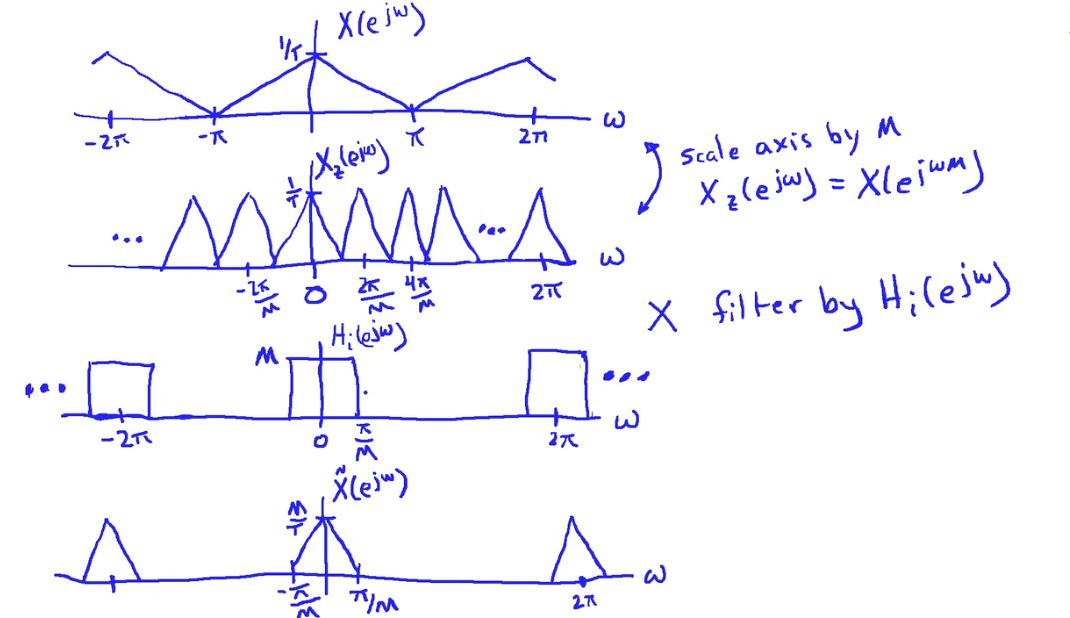
\includegraphics[width = 0.7\textwidth, frame]{Figures/Multirate/upsampling_example_spectrum}
\caption{Upsampling Example in DTFT spectrum}
\label{fig:Multirate:upsampling_example_spectrum}
\end{figure} 


\begin{itemize}

\item The spectrum at $\pi$ in $X(\omega_d)$ is now shown at $\displaystyle\frac{\pi}{M}$ in $X_z(\omega_d)$ 

\item We filter the signal $X_z(\omega_d)$ using a LPF 

\end{itemize}

%*****************************************************
%*****************************************************
%*****************************************************

\chapter{Multirate Sampling by Dr.Michael Lustig Berkely}


\section{Motivation}



\section{Downsampling}


\begin{itemize}

\item The input of the dowsampling operation is a discrete signal $x[k]$

\item What happens when we do dowsampling ?

The answer is in the spectrum.

\begin{itemize}
\item Recall that sampling in time give us replicate in frequency

\item DTFT for $x[k]$ and $x_{\text{decimated}}[k] \, = \, x[k \, M]$ where $M$ is the dowsampling factor


\item Equations:

\begin{equation}
\begin{array}{rcl}
X(\omega_d) \, &=& \, \displaystyle\frac{1}{T_s} \, \displaystyle\sum_n X_c \left[\, j \, \left(\, \omega_d \, - \, n \, \omega_s \,\right)  \,\right] \\ \\
X_{\text{decimated}}(\omega_d) \, &=& \, \displaystyle\frac{1}{M \, T_s} \, \displaystyle\sum_n X_c \left[\, j \, \left(\,  \displaystyle\frac{\omega_d}{M}  \, - \, n \,  \displaystyle\frac{\omega_s}{M} \,\right)  \,\right] 
\end{array}
\label{Eq:Multirate_Sampling_Decimation_spectrum_relation}
\end{equation}

Equation (\ref{Eq:Multirate_Sampling_Decimation_DTFT}) says that if we compress in time, we get more replicate in the frequency


\end{itemize}

\item Next step: is to find the relation between $X_{\text{DTFT}}(\omega_d) $ and $X_{\text{decimated}}(\omega_d) $ without using the CTFT spectrum $X_{\text{CTFT}}(\omega_c)$
	
	\begin{itemize}
	\item Relation:
	
	\begin{equation}
	\begin{array}{rcl}
		X_{\text{decimated}}(\omega_d) \, &=& \, \displaystyle	\frac{1}{M} \, \displaystyle\sum_{i \, = \, 0}^{M \, - \, 1} X_{\text{DTFT}} \left(\,  \displaystyle\frac{\omega_d}{M} \, - \, \displaystyle\frac{2 \pi}{M} \, i \,\right)   
	\end{array}	\label{Eq:Multirate_Sampling_Decimation_spectrum_dtft_relation}
	\end{equation}		
	
	\item Equation (\ref{Eq:Multirate_Sampling_Decimation_spectrum_dtft_relation}) tells us that our bandwidth will expand (stretch) by a factor of $M$.

	\end{itemize}


\end{itemize}



\section{Aliasing Revisited}

Recall that in aliasing , if we have $f \geq \, \displaystyle\frac{F_s}{2}$, then aliasing.\\

In undersampling (1 of Bandpass Sampling techinques:)

\begin{itemize}
    \item Rule: The sampled spectrum must fall in a 1 Nyqyuist Zone only
\end{itemize}


%\begin{figure}[h]
%\centering
%\includegraphics[width = 0.7\textwidth, frame]{Figures/Multirate/undersampling_Nyquist_zone}
%\caption{Upsampling Example in DTFT spectrum}
%\label{fig:Multirate:undersampling_Nyquist_zone}
%\end{figure} 

\underline{Note:} figure undersampling Nyquist zone not found


\section{Upsampling}

So much like digital to analog conversion (to a certain point they have similarities, but not the same).